% !TEX root = Hauptdatei.tex
\section{Entwicklung des neuen Konzepts}\label{hauptabschnitt_3}

%Vorgehensweise
%	Qualitätskriterien/Anforderungen ISO 25010
%	Entscheidungsbewertung
%	Design Patterns/Architectural Patterns
%	Auswahl HMI Tool
%Konzeptionierung
%	Gewählte Architektur
%	Gewählte Patterns (MVC)


%Dieses Kapitel beschäftigt sich mit der Entwicklung des neuen \ac{HMI}-Konzepts. In den nachfolgenden Kapiteln wird der Prozess der Softwarearchitektur, für diese Plattform, beschrieben.
%Bei der Entwicklung des neuen Konzepts müssen zu aller erst die Anforderungen an die Software identifiziert werden. Mit Hilfe der Anforderungen kann nach und nach ein Konzept entwickelt werden. \\

Dieses Kapitel beschäftigt sich mit der Entwicklung des neuen \ac{HMI}-Konzepts. In den nachfolgenden Kapiteln wird das Konzept für eine Softwarearchitektur entwickelt. Dabei müssen zuerst die Anforderungen an die Software identifiziert werden. Mit diesen Anforderungen werden im Anschluss Entwurfsmuster bewertet und ausgewählt und anschließend ein Architektur-Konzept erstellt.\\


\subsection{Gewichtung der ISO25010-Kriterien}
\label{Bewertung der ISO25010-Kriterien}
Die ersten Architekturtreiber sollen mit einer Entscheidungsbewertung herausgefunden werden. Dazu werden die ISO 25010 Kriterien von verschiedenen Mitarbeitern unabhängig gewichtet. Für die Gewichtung werden die Kriterien in eine Gegenüberstellungsmatrix eingefügt, welche dann von erfahrenen Mitarbeitern abgewogen werden.\\
  

\begin{figure}[htb]
	\centering
	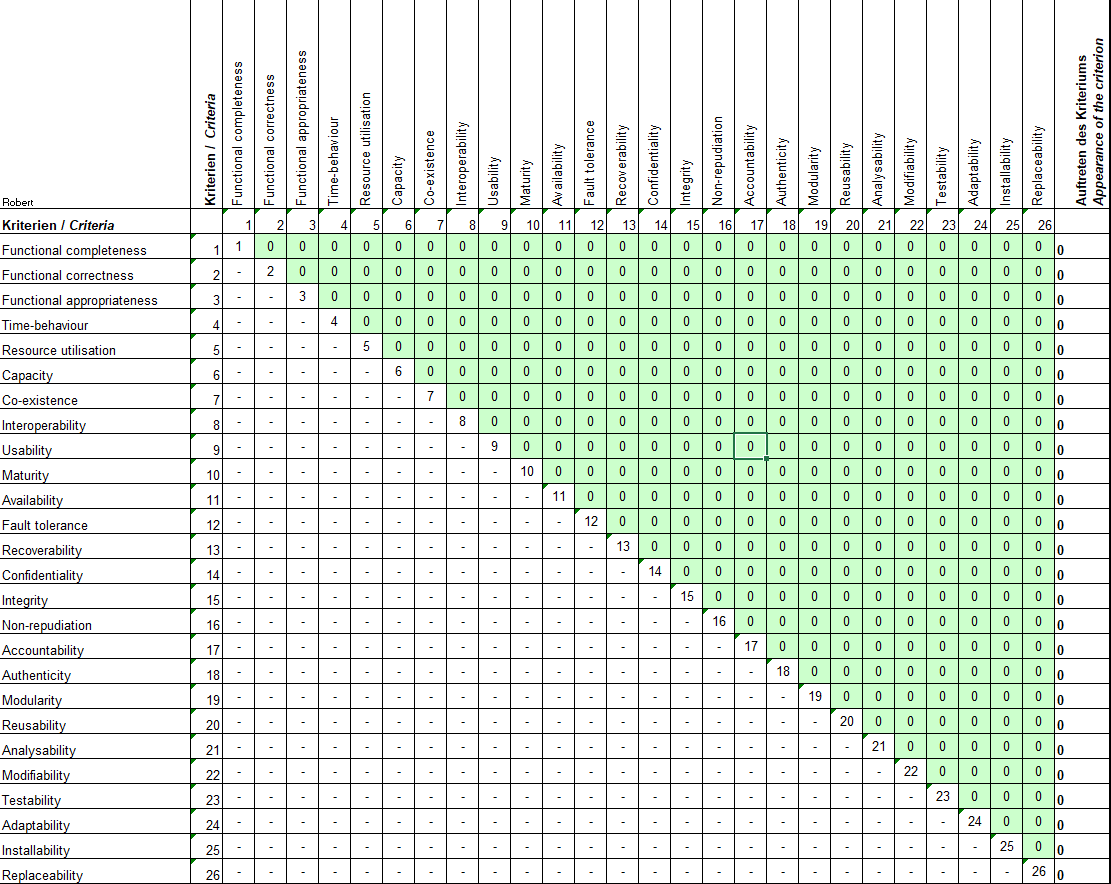
\includegraphics[width=\textwidth]{img/3_entwicklung_neues_kontept/Gewichtung}
	\caption{Gewichtungsmatrix der Qualitätskriterien nach ISO 25010}
	\label{fig:gewichtung}
\end{figure}
\newpage

Bei einer Gegenüberstellungsmatrix wird jedes Kriterium mit jedem anderen Kriterium verglichen.
Bei der Bewertung muss ausgewählt werden, welches Kriterium wichtiger ist. Die Matrix ist wie in Abbildung \ref{fig:gewichtung} aufgebaut. Die Kriterien stehen einmal in der vertikalen linken Spalte und einmal in der horizontalen Zeile in der gleichen Reihenfolge. In der Spalte daneben bzw. in der Zeile darunter bekommt jedes Kriterium eine fortlaufende Nummer, hier von 1 bis 26. In den Zellen in denen sich die gleichen Kriterien treffen wird direkt die Nummer des entsprechenden Kriteriums eingetragen, hier muss keine Entscheidung getroffen werden. Die eingetragenen Nummer bilden eine Diagonale durch die Matrix und teilt diese in zwei Hälften. Beide Hälften sind gleich, denn in beiden treffen sich jeweils alle Kriterien einmal. Daher muss nur die eine Hälfte ausgefüllt werden. Die obere rechte Hälfte wird zum Bewerten genutzt. Für die Bewertung muss dann in jede übrig gebliebene Zelle die Nummer des dominierenden Kriteriums eingetragen werden. Sind alle Zellen ausgefüllt ist in der rechten vertikalen Spalte das Ergebnis zu sehen. In dieser Spalte wird gezählt, wie oft ein Kriterium dominiert hat, das ist das Gewicht des Kriteriums.\\



\begin{table}[htb]
	\caption[Gesamtgewichtung]{Tabellarische Übersicht der Einzelgewichtungen der Qualitätskriterien}
	\label{tab:gewichtung}
	\centering
	\footnotesize
	\begin{tabular}{|l|c|c|c|c|c|}
		\hline
		                           & Architekt & SW-Entwickler & Kundensicht & Architekt & SW-Entwickler \\ \hline
		Functional completeness    &     5     &       1       &     15      &     1     &      11       \\ \hline
		Functional correctness     &    18     &      26       &     22      &    26     &      23       \\ \hline
		Functional appropriateness &     7     &      21       &     23      &    11     &      12       \\ \hline
		Time-behaviour             &    17     &      20       &     20      &    23     &      14       \\ \hline
		Resource utilisation       &    16     &      20       &     13      &    11     &       9       \\ \hline
		Capacity                   &     9     &      14       &     12      &     3     &       6       \\ \hline
		Co-existence               &     7     &      18       &      1      &     9     &      14       \\ \hline
		Interoperability           &     7     &       3       &     20      &    10     &      18       \\ \hline
		Usability                  &    10     &      17       &     16      &    15     &      14       \\ \hline
		Maturity                   &    24     &      16       &     16      &    24     &      24       \\ \hline
		Availability               &    18     &      14       &     18      &    24     &      26       \\ \hline
		Fault tolerance            &    24     &      22       &     16      &    13     &      22       \\ \hline
		Recoverability             &    23     &      13       &     14      &    16     &      22       \\ \hline
		Confidentiality            &    26     &      12       &     26      &    11     &      22       \\ \hline
		Integrity                  &    23     &      10       &     25      &    11     &      22       \\ \hline
		Non-repudiation            &     2     &       9       &      3      &     7     &      10       \\ \hline
		Accountability             &    14     &       9       &      4      &     6     &       6       \\ \hline
		Authenticity               &    16     &       8       &      5      &     6     &       9       \\ \hline
		Modularity                 &    15     &      24       &     10      &    18     &      17       \\ \hline
		Reusability                &    15     &       6       &      8      &    17     &      17       \\ \hline
		Analysability              &     5     &       7       &      5      &    19     &      11       \\ \hline
		Modifiability              &    11     &      23       &      9      &    20     &       9       \\ \hline
		Testability                &    18     &      24       &     24      &    22     &       5       \\ \hline
		Adaptability               &     7     &       5       &      3      &    21     &       5       \\ \hline
		Installability             &     2     &       4       &      7      &     4     &       2       \\ \hline
		Replaceability             &    12     &       3       &     15      &     3     &       1       \\ \hline
	\end{tabular}
\end{table}

Die Bewertung wurde insgesamt von fünf Personen aus unterschiedlichen Bereichen durchgeführt. Zu den verschiedenen Bereichen zählen zum einen zwei Software-Archi"=tekten, zwei Softwareentwickler und ein Akquisemitarbeiter für die Kundensicht. Diese Verteilung gibt eine gute Gesamtübersicht. Von der Systemplanung, über die Durchführung, bis hin zum Kunden sind dadurch alle Ansichten vertreten.
Das Ergebnis ist in Tabelle \ref{tab:gewichtung} dargestellt. \\
%Aus den unterschiedlichen Gewichtungen der Befragten wird eine Gesamtgewichtung berechnet. Hierzu wird der Durchschnitt genommen. Mit Hilfe der Gesamtgewichtung werden passende Entwurfsmuster ausgewählt die, die wichtigsten Qualitätskriterien weitstgehend erfüllen. Durch die Eingrenzung der möglichen Entwurfsmuster ist es leichter ein Architektur zu erstellen, da der Fokus auf ein paar wenige Entwurfsmuster gelegt werden kann.\\

Aus den Einzelgewichtungen der fünf Experten wird eine Gesamtgewichtung erstellt, dazu wird der Durchschnitt für jedes Kriterium berechnet. Das Ergebnis ist in Tabelle \ref{tab:gesamtgewichtung} zu sehen. Mit Hilfe dieser Tabelle können verschieden Entwurfsmuster bewertet werden.

\begin{table}[htb]
	\caption[Gesamtgewichtung]{Durchnittliche Gewichtung der ISO-Kriterien (sortiert nach Gewichtung)}
	\label{tab:gesamtgewichtung}
	\centering
	\small
	\begin{tabular}{|l|c|}
		\hline
		                           & Gesamt \\ \hline
		Functional correctness     &   23   \\ \hline
		Maturity                   &   21   \\ \hline
		Availability               &   20   \\ \hline
		Time-behaviour             &   19   \\ \hline
		Testability                &   19   \\ \hline
		Fault tolerance            &   19   \\ \hline
		Confidentiality            &   19   \\ \hline
		Recoverability             &   18   \\ \hline
		Integrity                  &   18   \\ \hline
		Modularity                 &   17   \\ \hline
		Functional appropriateness &   15   \\ \hline
		Usability                  &   14   \\ \hline
		Resource Utilisation       &   14   \\ \hline
		Modifiability              &   14   \\ \hline
		Reusability                &   13   \\ \hline
		Interoperability           &   12   \\ \hline
		Co-Existence               &   10   \\ \hline
		Capacity                   &   9    \\ \hline
		Authenticity               &   9    \\ \hline
		Analysability              &   9    \\ \hline
		Adaptability               &   8    \\ \hline
		Accountability             &   8    \\ \hline
		Replaceability             &   7    \\ \hline
		Functional Completeness    &   7    \\ \hline
		Non-Repudiation            &   6    \\ \hline
		Installability             &   4    \\ \hline
	\end{tabular}
\end{table}

%Einige der Kriterien sind für das Architektur-Konzept nicht relevant. Functional correctness 
\newpage
\subsection{Sammlung und Bewertung von Entwurfsmustern}
\label{Sammlung und Bewertung von Entwurfsmustern}
Damit Entwurfsmuster für die Architektur ausgewählt werden können, müssen zuerst Entwurfsmuster gesammelt und bewertet werden.\\

Bei der Recherche wurde der Fokus darauf gelegt, Entwurfsmuster im Zusammenhang mit den ISO-Kriterien zu finden. Da mit diesen Kriterien die Entwurfsmuster bewertet werden sollen. Aus der Recherche ergaben sich zwei wissenschaftliche Arbeiten die sich mit diesem Thema beschäftigten. Die erste Arbeit ist von 2006 mit dem Titel \glqq Towards a Maintainability Evaluation in Software Architectures \grqq \cite{towards_maintain} und die andere Arbeit von 2019 mit dem Titel \glqq Design Patterns for Software Evolution Requirements \grqq \cite{SW_evol_req}. Auf diese zwei Arbeiten wird in diesem Kapitel wesentlich Bezug genommen. Zusätzlich ergab die Recherche einen Report über sichere Entwurfsmuster, mit dem Titel \glqq Secure Design Patterns \grqq \cite{DoughertySecureDesign2009}.

\begin{figure}[htb]
	\centering
	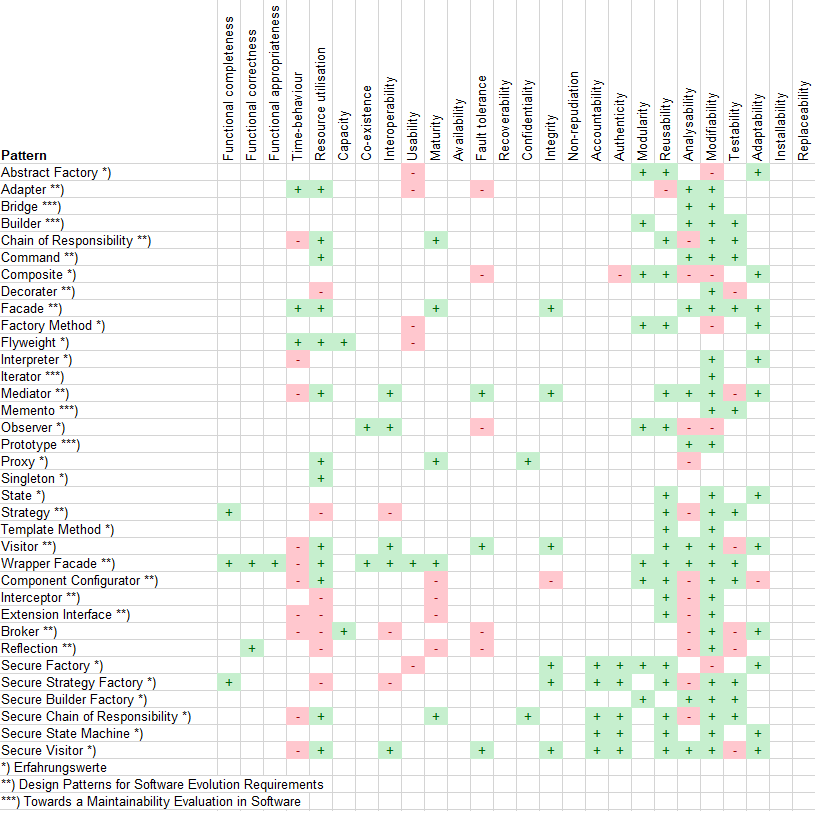
\includegraphics[width=14.5cm]{img/3_entwicklung_neues_kontept/Pattern_Sammlung_neu}
	\caption{Matrix der Entwurfsmuster und ISO-Kriterien}
	\label{fig:pattern_sam}
\end{figure}

Die ersten beiden Arbeiten beziehen sich vorwiegend auf die Standard-\ac{GoF}-Ent"=wurfs"=muster. Die letzte Arbeit hat die \ac{GoF}-Muster, unter dem Aspekt der Sicherheit, weiterentwickelt. Der Übersichtlichkeit wegen, wurden die Daten in eine Tabelle übertragen. Abbildung \ref{fig:pattern_sam} zeigt das Ergebnis. Die linke Spalte enthält alle gefundenen Entwurfsmuster in den Arbeiten und zusätzlich die \ac{GoF}-Entwurfsmuster, welche in keiner Arbeit erwähnt wurden. Die linke Spalte beinhaltet alle gefunden Entwurfsmuster. Die oberste Zeile enthält die ISO-25010 Kriterien. Dadurch ergibt sich eine Matrix, in der mit einem Plus, einem Minus, oder einer leeren Zelle das Entwurfsmuster in Bezug auf ein Kriterium bewertet werden kann. \\

\subsection{Auswahl Entwurfsmuster}
%Auswahl der Entwurfsmuster auf Basis der Entscheidungsbewertung

In diesem Kapitel werden die Ergebnisse aus Kapitel \ref{Bewertung der ISO25010-Kriterien} und Kapitel \ref{Sammlung und Bewertung von Entwurfsmustern} zusammengeführt. Die Entwurfsmuster werden in einer Matrix den ISO-Kriterien gegenübergestellt. Das Ergebnis ist eine Punktzahl für jedes Entwurfsmuster im Hinblick auf die ISO-Kriterien. Mit Hilfe der Punktzahl lässt sich feststellen, welche Entwurfsmuster am Besten zu der Gewichtung der Qualitätskriterien passen und worauf besonders geachtet werden sollte.\\

Die Punktzahl wird nach Gleichung 1 berechnet: Ein Minus in der Entwurfsmusterbewertung, heißt das Ergebnis der ISO-Bewertung wird mal eins genommen. Eine leere Zelle in der Entwurfsmusterbewertung, bedeutet das Ergebnis der ISO-Bewertung wird mal zwei genommen. Ein plus, heißt das Ergebnis der ISO-Bewertung wird mal drei genommen. Anschließend werden die Punktzahlen über alle Kriterien aufsummiert.\\

\begin{align}
	X &= \sum_{i=1}^{31} k_i\cdot z
\end{align}
\begin{align*}
	&X = \text{Punktzahl für Reihenfolge} \\
	&k_i = \text{Durchschnittsgewicht Kriterium 1 bis 31} \\
	&z = \text{1..3}
\end{align*}

Die Entwurfsmuster werden anschließend nach der erreichten Punktzahl sortiert. Daraus ergibt sich Tabelle \ref{tab:reihenfolge_pattern} mit der Reihenfolge der Entwurfsmuster.

\begin{table}[hp]
	\caption[Reihenfolge Entwrufsmuster]{Reihenfolge der Entwurfsmuster von oben (beste Punktzahl) nach unten (niedrigste Punktzahl)}
	\label{tab:reihenfolge_pattern}
	\centering
	\small
	\begin{tabular}{|l|c|l|}
		\hline
		Entwurfsmuster                 & Punktzahl & geeignet für      \\ \hline
		Command                        &   1520    & -                 \\ \hline
		Secure Chain of Responsibility &   1520    & -                 \\ \hline
		Wrapper Facade                 &   1504    & View              \\ \hline
		Memento                        &   1491    & View              \\ \hline
		Strategy                       &   1457    & View              \\ \hline
		Interpreter                    &   1446    & -                 \\ \hline
		Proxy                          &   1441    & View              \\ \hline
		Bridge                         &   1428    & View              \\ \hline
		Extension Interface            &   1393    & -                 \\ \hline
		Facade                         &   1376    & View              \\ \hline
		Secure Factory                 &   1302    & MVC               \\ \hline
		Secure Visitor                 &    790    & -                 \\ \hline
		Mediator                       &    773    & -                 \\ \hline
		Visitor                        &    773    & -                 \\ \hline
		Builder                        &    763    & -                 \\ \hline
		Secure Builder Factory         &    763    & -                 \\ \hline
		Chain of Responsibility        &    757    & -                 \\ \hline
		Secure Strategy Factory        &    757    & -                 \\ \hline
		Secure State Machine           &    756    & Controller        \\ \hline
		State                          &    739    & Controller        \\ \hline
		Flyweight                      &    732    & -                 \\ \hline
		Template Method                &    731    & -                 \\ \hline
		Prototype                      &    727    & -                 \\ \hline
		Iterator                       &    718    & -                 \\ \hline
		Singleton                      &    718    & Controller, Model \\ \hline
		Abstract Factory               &    714    & MVC               \\ \hline
		Adapter                        &    714    & -                 \\ \hline
		Factory Method                 &    714    & MVC               \\ \hline
		Observer                       &    714    & Model, View       \\ \hline
		Component Configurator         &    706    & -                 \\ \hline
		Compisite                      &    691    & -                 \\ \hline
		Interceptor                    &    687    & -                 \\ \hline
		Decorator                      &    685    & -                 \\ \hline
		Reflection                     &    659    & -                 \\ \hline
		Broker                         &    643    & -				   \\ \hline
	\end{tabular}
\end{table}
\newpage

In der Tabelle sind alle recherchierten Entwurfsmuster aufgelistet und sortiert nach der erreichten Punktzahl. In der rechten Spalte ist außerdem aufgeführt, für welchen Teil des Model-View-Controller das Entwurfsmuster geeignet ist. Da nicht jedes Muster zwangsläufig verwendet werden kann gibt es auch Zeilen ohne Eintrag. Im oberen Teil der Tabelle sind die meisten Entwurfsmuster der View zugeordnet. Daraus lässt sich schließen, dass der View den größten Teil der Aufmerksamkeit zu widmen ist.\\

\subsection{Architektur}
%Endgültige Architektur UML-Diagramme usw...

In diesem Kapitel wird die vorläufige Software-Architektur für das Proof-Of-Concept entwickelt. Die Architektur ist in diesem Fall noch nicht an die Eigenschaften von eventuellen \ac{HMI} Frameworks angepasst. Eine weitere Anpassung nach Auswahl des \ac{HMI}-Frameworks ist notwendig.\\

\glqq{}We need SMART Models, THIN Controllers, and DUMB Views\grqq{} \cite{mvc_wiki}. Dem entsprechend sollte der größte Teil der Komplexität im Model umgesetzt werden. Bei bisheriger Software lag der Hauptteil der Komplexität aber in den ViewControllern, also in der View. Der Controller sollte wirklich nur die Zustände verwalten und View sollte so wenig Komplexität beinhalten wie möglich. Das größte Augenmerk in der Entwicklung muss daher auf das Model gelegt werden. Der Controller und die View sollten schmal bleiben. Ziel sollte es sein, dass die Aufgaben im MVC-Muster strikt getrennt bleiben. Aufgrund des aktuell eingesetzten \ac{HMI} Frameworks konnte das \ac{MVC}-Muster nicht immer korrekt eingehalten werden.\\

In den folgenden Kapitel wird auf dieser Basis und den ausgewählten Entwufsmuster das Softwarearchitekturkonzept mit Hilfe von UML-Diagrammen erarbeitet.\\

\subsubsection{Model}
Das Model setzt sich aus dem Singleton-, Fabrik- und Beobachter-Entwurfsmuster zusammen. Das Singleton-Entwurfsmuster stellt sicher, dass eine Klasse nicht mehrfach instanziiert wird. Eine Mehrfachinstantiierung des Models würde Asynchronität der Daten und einen enormen Ressourcenverbrauch mit sich bringen. Das Singleton wird als abstrakte Klasse umgesetzt und das Model erbt von der Klasse Singleton. Die Fabrik kümmert sich um die Erstellung und Verwaltung vom Model. Die Verbindung zwischen Model und View bzw. Controller stellt das Beobachter-Muster her. Das Beobachter-Muster ermöglicht den Datenaustausch zwischen zwei oder mehr Objekten, verhindert aber gleichzeitig eine zu starke Kopplung der beteiligten Objekte. Die Implementierung des Beobachtermusters ist sehr stark vom verwendeten Framework abhängig.\\

Abbildung \ref{fig:model_diagram} veranschaulicht einen beispielhaften Entwurf des Models. Die in Abbildung \ref{fig:model_diagram} entworfenen Klassen sind als Beispiel zu verstehen und werden kundenspezifisch realisiert.\\

\begin{figure}[htb]
	\centering
	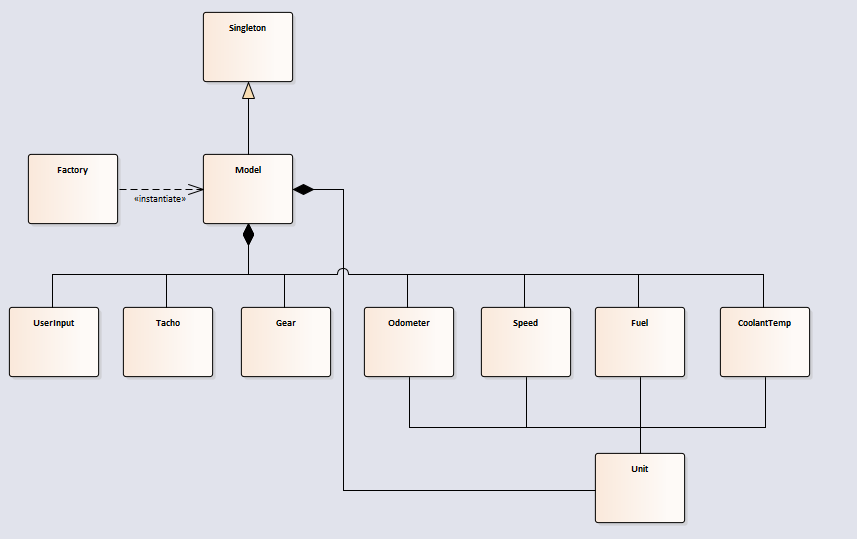
\includegraphics[width=\textwidth]{img/3_entwicklung_neues_kontept/model_diagram}
	\caption{UML-Diagramm des Model}
	\label{fig:model_diagram}
\end{figure}

In den einzelnen Modulen muss zunächst geprüft werden, ob erhaltene Werte plausibel sind. Nach der Plausibilisierung wird überprüft ob eine Umrechnung der Werte in eine andere Einheit notwendig ist. Nachdem alle Überprüfungen und Umrechnungen abgeschlossen sind, kann der Wert an die View weitergegeben werden.\\

Das Model soll so flexibel wie möglich sein und gleichzeitig Entwicklungsaufwand einsparen. Daher ist jede Klasse unabhängig von den anderen Klassen und kann jederzeit entfernt oder hinzugefügt werden. Der Vorteil von diesem Ansatz ist die hohe Modularität und die Möglichkeit große Teile des Models wiederzuverwenden. Dieser Ansatz kann im späteren Verlauf ein einfaches zusammenstellen des Models ermöglichen. Mit Hilfe eines Formulars könnten einzelne Module nach Kundenwunsch ausgewählt werden. Das Model wird dann durch ein Skript zusammengefügt und bereitgestellt.\\ 

\subsubsection{View}
Die konkrete Umsetzung der View hängt stark mit dem verwendeten HMI Framework zusammen und wird teilweise sogar vorgegeben.\\

Kapitel \ref{hauptabschnitt_4} beschäftigt sich mit der Evaluation dieser \ac{HMI} Frameworks und deren Einfluss auf eine Softwarearchitektur einer \ac{HMI}.\\

\subsubsection{Controller}
Der Controller besteht aus dem Singleton-, Zustand-, Fabrik- und Beobachter-Muster. Der Controller wird ebenfalls als Singleton realisiert, damit keine doppelten Zustände existieren und Ressourcen geschont werden. Im Controller ist jeder mögliche Zustand als konkrete Klasse realisiert. Die konkreten Zustände sind von der abstrakten Klasse Zustand abgeleitet. Die Fabrik kümmert sich auch hier um die Erstellung und Verwaltung des Controllers. Das Beobachter-Muster ist der Gegenpart zum Beobachter-Muster im Model. Das Model stellt die Daten bereit und der Controller verarbeitet die Daten und prüft einen möglichen Zustandswechsel. \\

Abbildung \ref{fig:controller_diagram} zeigt einen beispielhaften Entwurf eines Controllers. Die In Abbildung \ref{fig:controller_diagram} zu sehenden Zustände sollen als Beispiel verstanden werden und müssen kundenspezifisch durch konkrete Zustände ersetzt werden.\\

\begin{figure}[htb]
	\centering
	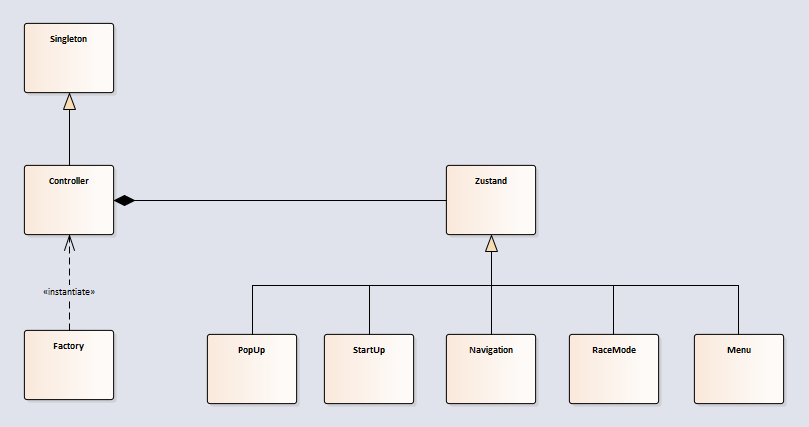
\includegraphics[width=\textwidth]{img/3_entwicklung_neues_kontept/controller_diagram}
	\caption{UML-Diagramm des Controllers}
	\label{fig:controller_diagram}
\end{figure}

Im Controller dürfen keine Berechnungen oder ähnliches stattfinden, es muss immer klar sein welcher Zustand der Aktuelle ist. Hier können ebenfalls Zustände beliebig hinzugefügt oder entfernt werden. Das ermöglicht auch hier, dass die Zustände in einem Formular ausgewählt werden können und anschließend durch ein Skript zusammengestellt wird.\\




